% gc-09-Analyzing.tex

\documentclass[xcolor=dvipsnames]{beamer}
\usepackage{teachbeamer}
\newcommand{\hohq}{Jane}
\newcommand{\wili}{She}
\newcommand{\ahhi}{she}
\newcommand{\usax}{13}
\newcommand{\bohh}{her}
\newcommand{\reeq}{2.5}
\newcommand{\aeza}{8.3}
\newcommand{\emah}{2.1}
\newcommand{\biet}{4.9}

\title{Optimization and Analyzing Functions}
\subtitle{{\CourseNumber}, BCIT}

\author{\CourseName}

\date{February 5, 2018}

% \begin{figure}[h]
% 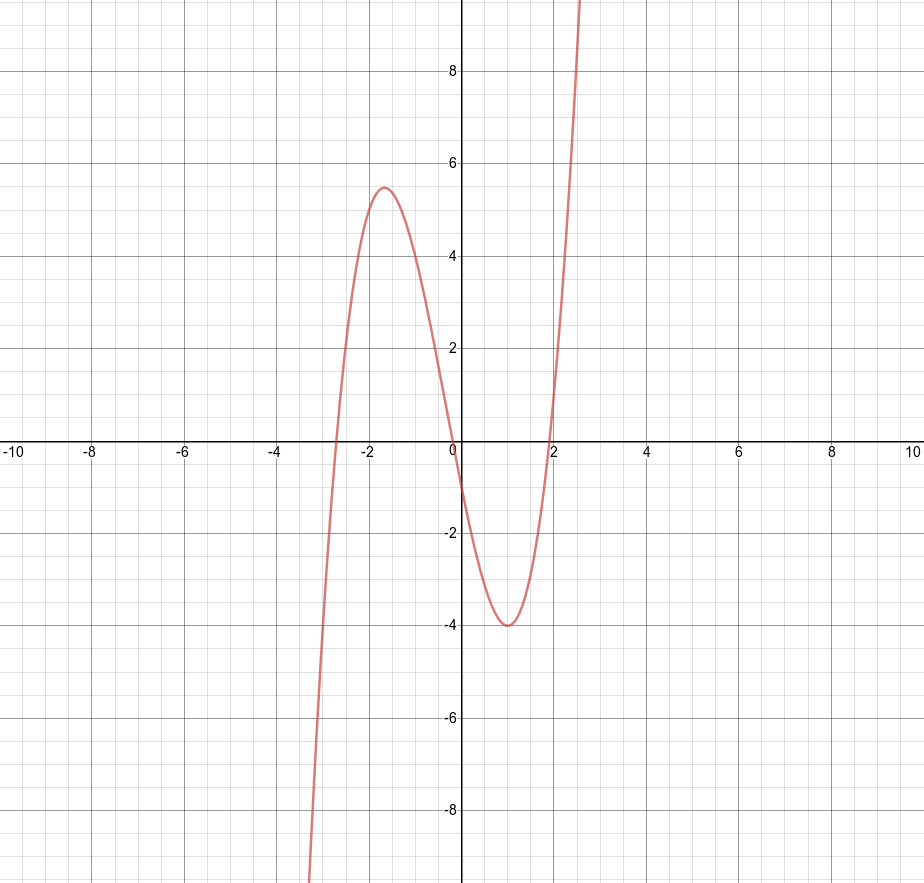
\includegraphics[scale=.3]{./diagrams/extrema1.png}
% \end{figure}

\begin{document}

\begin{frame}
  \titlepage
\end{frame}

\begin{frame}
  \frametitle{Relative Extrema}
A function $f$ has a \alert{relative maximum} at $x=c$ if there exists
an open interval $(a,b)$ containing $c$ such that $f(x)\leq{}f(c)$ for
all $x$ in $(a,b)$.

\bigskip

A function $f$ has a \alert{relative minimum} at $x=c$ if there exists
an open interval $(a,b)$ containing $c$ such that $f(x)\geq{}f(c)$ for
all $x$ in $(a,b)$.
\end{frame}

\begin{frame}
  \frametitle{Derivatives and Extrema}
  At any number $c$ where a differentiable function $f$ has a relative
  extremum, $f'(c)=0$. The converse is not true. Consider the
  following two functions and their derivatives.
\begin{equation}
  \label{eq:thapoich}
f_{1}(x)=x^{3}+x^{2}-5x-1
\end{equation}
\begin{equation}
  \label{eq:gohshaem}
f_{2}(x)=\left(\frac{3}{10}x\right)^{3}
\end{equation}
\end{frame}

\begin{frame}
  \frametitle{Derivatives and Extrema Graph I}
  \begin{figure}[h]
    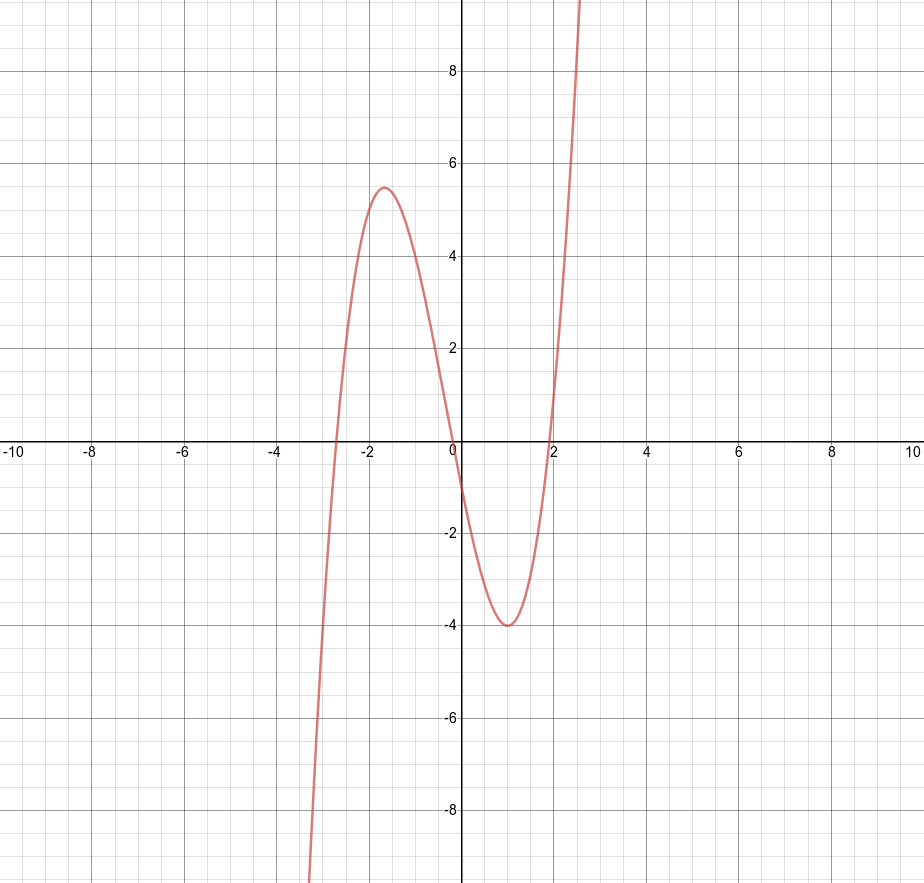
\includegraphics[scale=.3]{./diagrams/extrema1.png}
  \end{figure}
\end{frame}

\begin{frame}
  \frametitle{Derivatives and Extrema Graph II}
  \begin{figure}[h]
    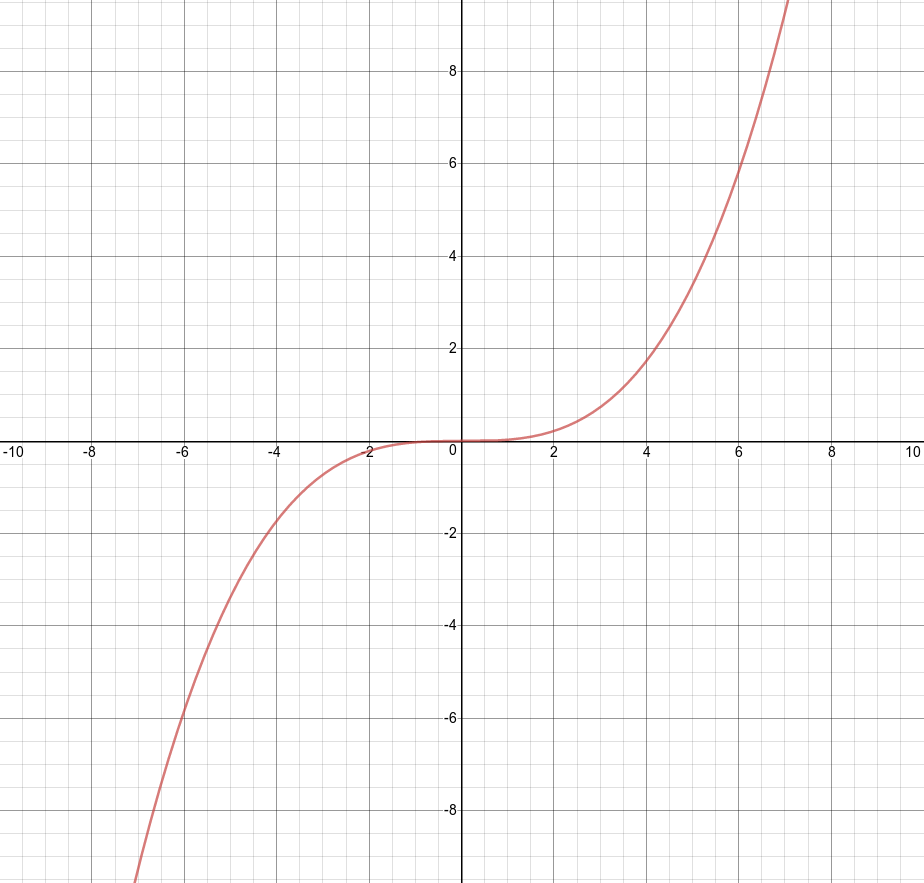
\includegraphics[scale=.3]{./diagrams/extrema2.png}
  \end{figure}
\end{frame}

\begin{frame}
  \frametitle{Derivatives and Extrema Caution}
Note that a function may have an extremum at a point where the
derivative is not $0$ if at that point the function is not
differentiable. Consider this function and its derivative.
\begin{equation}
  \label{eq:ceezukoh}
f_{3}(x)=x^{\frac{2}{3}}
\end{equation}
\begin{block}{Critical Number}
  A \alert{critical number} of a function $f$ is any number $x$ in the
  domain of $f$ such that $f'(x)=0$ or $f'(x)$ does not exist.
\end{block}
\end{frame}

\begin{frame}
  \frametitle{Derivatives and Extrema Graph III}
  \begin{figure}[h]
    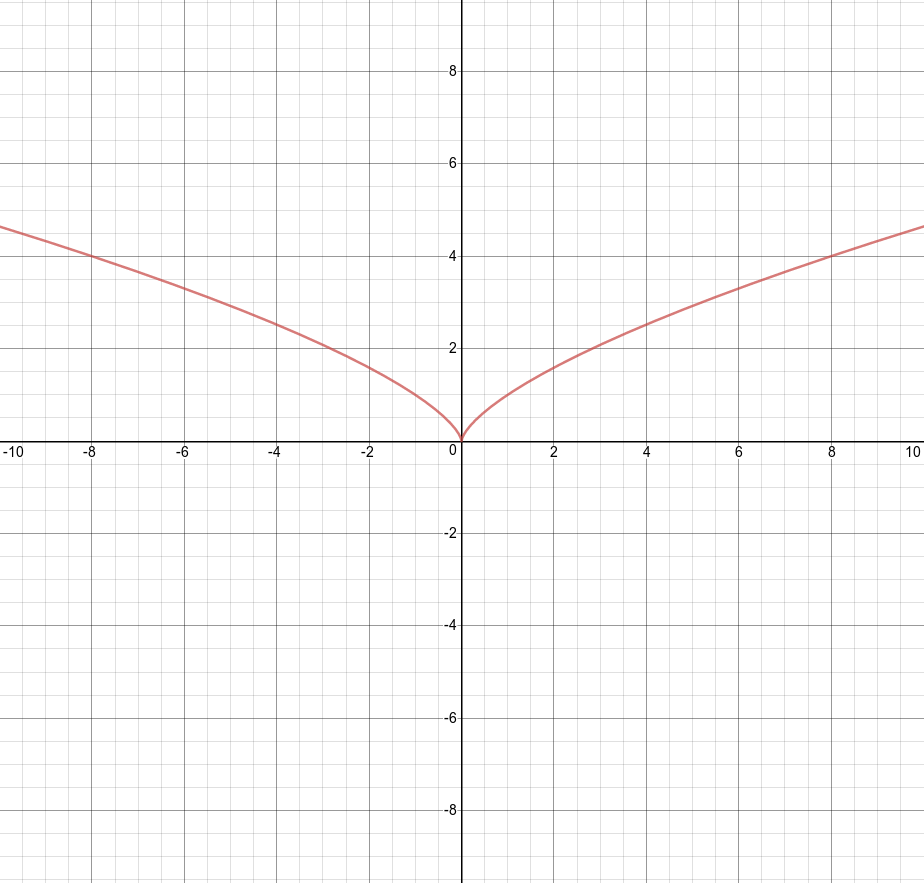
\includegraphics[scale=.3]{./diagrams/extrema3.png}
  \end{figure}
\end{frame}

\begin{frame}
  \frametitle{Critical Points and Extrema}
  \begin{figure}[h]
    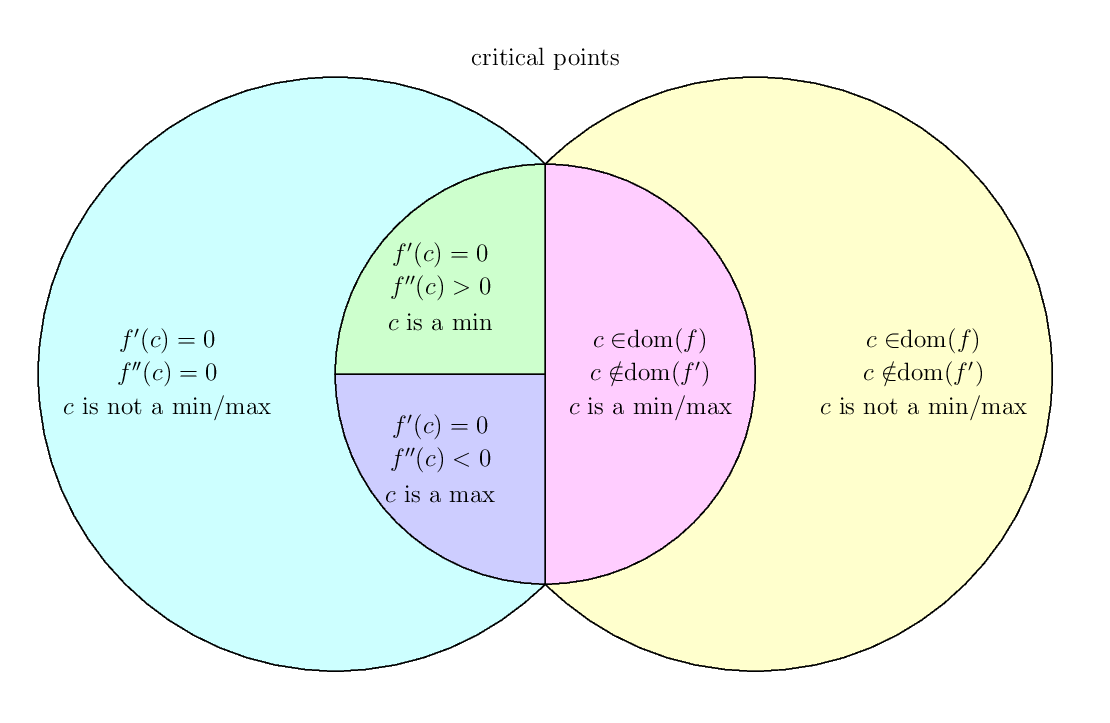
\includegraphics[scale=.3]{./diagrams/opt.png}
  \end{figure}
\end{frame}

\begin{frame}
  \frametitle{Critical Points Exercises}
{\ubung} Find the critical points of the following function,
\begin{equation}
  \label{eq:xoongohh}
f(x)=x^{3}-4x
\end{equation}
\end{frame}

\begin{frame}
  \frametitle{Critical Points Exercises}
{\ubung} Find the critical points of the following function,
\begin{equation}
  \label{eq:aghuomoh}
h(t)=-t^{2}+6t+6
\end{equation}
\end{frame}

\begin{frame}
  \frametitle{Critical Points Exercises}
{\ubung} Find the critical points of the following function,
\begin{equation}
  \label{eq:yakovuap}
f(x)=\frac{1}{2}x^{4}-x^{2}
\end{equation}
\end{frame}

\begin{frame}
  \frametitle{Critical Points Exercises}
{\ubung} Find the critical points of the following function,
\begin{equation}
  \label{eq:aweefahx}
g(x)=\frac{x+1}{x}
\end{equation}
\end{frame}

\begin{frame}
  \frametitle{Critical Points Exercises}
{\ubung} Find the critical points of the following function,
\begin{equation}
  \label{eq:ebukatio}
f(x)=x\sqrt{x-4}
\end{equation}
\end{frame}

\begin{frame}
  \frametitle{Critical Points Exercises}
{\ubung} Find the critical points of the following function,
\begin{equation}
  \label{eq:imeecohd}
f(x)=2\tan{}x-\tan^{2}x
\end{equation}
\end{frame}

\begin{frame}
  \frametitle{Critical Points Exercises}
{\ubung} Find the critical points of the following function,
\begin{equation}
  \label{eq:inaidimo}
h(s)=s^{\frac{5}{3}}
\end{equation}
\end{frame}

\begin{frame}
  \frametitle{Extrema Exercises}
{\ubung} Find local maxima and minima for the following function:
\begin{equation}
  \label{eq:xxyxx1}
f(x)=3x^{3}-12x+5
\end{equation}
\end{frame}

\begin{frame}
  \frametitle{Extrema Exercises}
{\ubung} Find local maxima and minima for the following function:
\begin{equation}
  \label{eq:xxyxx2}
f(x)=\frac{x}{x^{2}+1}
\end{equation}
\end{frame}

\begin{frame}
  \frametitle{Extrema Exercises}
{\ubung} Find local maxima and minima for the following function:
\begin{equation}
  \label{eq:xxyxx3}
f(t)=t\sqrt{4-t^{2}}
\end{equation}
\end{frame}

\begin{frame}
  \frametitle{Extrema Exercises}
{\ubung} Find local maxima and minima for the following function:
\begin{equation}
  \label{eq:xxyxx4}
g(t)=\sqrt[3]{t}(8-t)
\end{equation}
\end{frame}

\begin{frame}
  \frametitle{Extrema Exercises}
{\ubung} Find local maxima and minima for the following function:
\begin{equation}
  \label{eq:xxyxx5}
g(t)=\cos{}t+\sin{}t
\end{equation}
\end{frame}

\begin{frame}
  \frametitle{Extrema Exercises}
{\ubung} Find local maxima and minima for the following function:
\begin{equation}
  \label{eq:xxyxx6}
f(x)=\ln(x^{2}+x+1)
\end{equation}
\end{frame}

\begin{frame}
  \frametitle{Extrema Exercises}
{\ubung} Find local maxima and minima for the following function:
\begin{equation}
  \label{eq:xxyxx7}
f(x)=\ln\left(\cos{}x\right)
\end{equation}
\end{frame}

\begin{frame}
  \frametitle{Optimization Word Problems}
% William Anthony Granville, page 116
{\ubung} Find the altitude of the cylinder of maximum volume that can
be inscribed in a given right cone.
  \begin{figure}[h]
    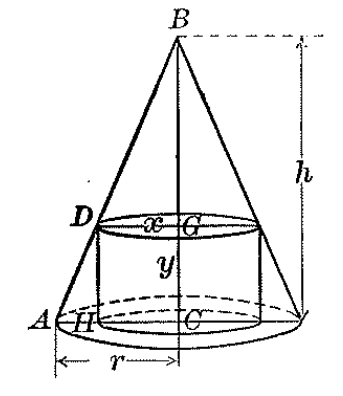
\includegraphics[scale=.3]{./diagrams/optcone.png}
  \end{figure}
\end{frame}

\begin{frame}
  \frametitle{Optimization Word Problems}
  {\ubung} A water tank is to be constructed with a square base and
  open top and is to hold 64 cubic yards. If the cost of the sides is
  \$1 a square yard, and of the bottom \$2 a square yard, what are the
  dimensions when the cost is a minimum? What is the minimum cost?
\end{frame}

\begin{frame}
  \frametitle{Optimization Word Problems}
  % William Anthony Granville, page 120
  % For solution consult Schmierbuch pages 2524ff
  {\ubung} The lower corner of a leaf, whose width is $a$, is folded
  over so as just to reach the inner edge of the page.
  \begin{enumerate}
  \item Find the width of the part folded over when the length of the
    crease is a minimum.
  \item Find the width when the area folded over is a minimum.
  \end{enumerate}
  \begin{figure}[h]
    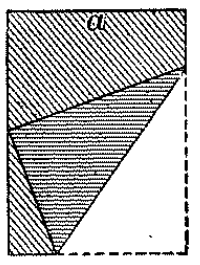
\includegraphics[scale=.4]{./diagrams/optleaf.png}
  \end{figure}
\end{frame}

\begin{frame}
  \frametitle{Optimization Word Problem Solution}
  \begin{figure}[h]
    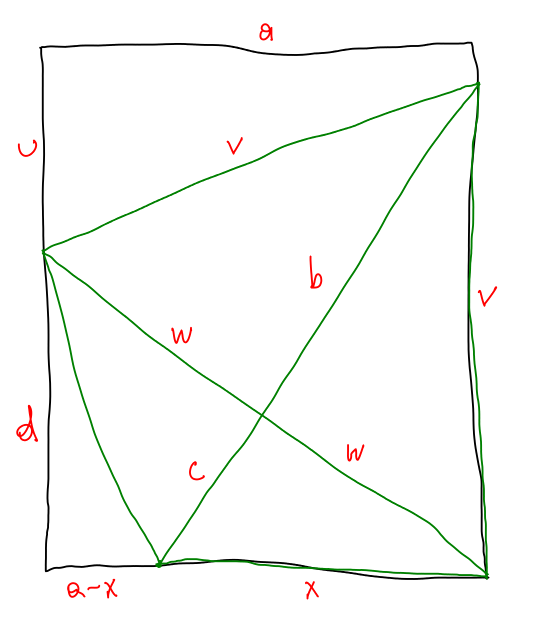
\includegraphics[scale=.35]{./diagrams/optleafsol.png}
  \end{figure}
\end{frame}

\begin{frame}
  \frametitle{Optimization Word Problem Solution}
Define a function $f(x)=b+c$. We want to minimize $f$ on the interval
$(\frac{a}{2},a]$. Notice that $b^{2}=v^{2}-w^{2}$ and
$c^{2}=x^{2}-w^{2}$. We need to express $v$ and $w$ by $x$ and the
fixed number $a$. From
\begin{equation}
  \label{eq:jaithean}
  \left(2w\right)^{2}=d^{2}+a^{2}
\end{equation}
we get
\begin{equation}
  \label{eq:ukohyaej}
  w^{2}=\frac{ax}{2}
\end{equation}
From
\begin{equation}
  \label{eq:loocootu}
  v^{2}=a^{2}+u^{2}
\end{equation}
we get
\begin{equation}
  \label{eq:zoojeefo}
  v^{2}=\frac{ax^{2}}{2x-a}
\end{equation}
\end{frame}

\begin{frame}
  \frametitle{Optimization Word Problem Solution}
  Consequently, the function to differentiate is
  \begin{equation}
    \label{eq:eeguyeex}
    f(x)=\frac{1}{\sqrt{2}}\left(\sqrt{\frac{a^{2}x}{2x-a}}+\sqrt{x(2x-a)}\right)
  \end{equation}
  After differentiation, it turns out that $f'(x)=0$ if and only if
  \begin{equation}
    \label{eq:shohyoom}
    x=\frac{3}{4}a
  \end{equation}
  This answers the first question. The answer for the second question is
  \begin{equation}
    \label{eq:zieshaiv}
    x=\frac{2}{3}a
  \end{equation}
\end{frame}

\begin{frame}
  \frametitle{Optimization Word Problems}
  {\ubung} A submarine telegraph cable consists of a core of copper
  wires with a covering made of nonconducting material. If $x$ denotes
  the ratio of the radius of the core to the thickness of the
  covering, it is known that the speed of signaling varies as
  \begin{equation}
    \label{eq:ehielush}
    x^{2}\ln\frac{1}{x}
  \end{equation}
Show that the greatest speed is attained when $x=\frac{1}{\sqrt{e}}$.
\end{frame}

\begin{frame}
  \frametitle{Optimization Word Problems}
  {\ubung} {\hohq} is {\reeq} miles offshore in a boat and wishes to
  reach a coastal village {\aeza} miles down a straight shoreline from
  the point nearest the boat. {\wili} can row {\emah} miles per hour
  and can walk {\biet} miles per hour. Where should {\ahhi} land
  {\bohh} boat to reach the village in the least amount of time?
\end{frame}

\begin{frame}
  \frametitle{Analyzing Functions I}
To analyze a function, determine the following features:
\begin{itemize}
\item Domain and range of the function.
\item Zeros (also called $x$-intercepts) of the function.
\item Critical points, maxima, minima.
\item Inflection points.
\item Asymptotes.
\item Is the function even ($f_{1}(x)=x^{2}+1$) or odd ($f_{2}(x)=x^{3}-x$)?
\end{itemize}
\end{frame}

\begin{frame}
  \frametitle{Analyzing Functions Step-By-Step I}
Here is a step-by-step guide to analyzing functions.
\begin{enumerate}
\item Determine the $x$-intercepts (also called zeros). Set $f(x)=0$
  and find the solution set.
\item Determine the critical points. Find the derivative $f'(x)$ and
  check whether there are points in the domain of $f$ that are not in
  the domain of $f'$. Then set $f'(x)=0$ and find the solution set.
\item Determine whether the critical points are maxima or minima or
  neither. Find $f''(x)$ and check whether $f''$ at the critical
  points is positive, negative, or neither. 
\end{enumerate}
\end{frame}

\begin{frame}
  \frametitle{Analyzing Functions Step-By-Step II}
Here is a step-by-step guide to analyzing functions.
\begin{enumerate}
\setcounter{enumi}{3}
\item Determine the inflection points. Set $f''(x)=0$ and find the
  solution set.
\item Determine the asymptotes. See next slide.
\item Determine whether, for all $x$ in the domain of $f$,
  $f(x)-f(-x)=0$ (in which case $f$ is even) or $f(x)+f(-x)=0$ (in
  which case $f$ is odd).
\item Using the information you have, and possibly a table of function
  values, graph the function. Then determine the domain and range of
  $f$.
\end{enumerate}
\end{frame}

\begin{frame}
  \frametitle{Finding Asymptotes I}
An asymptote is a linear function ($y=kx+d$ with slope $k$ and
$y$-intercept $d$) which the function graph of $f$ approaches. There
are three kinds of asymptotes.
\begin{block}{Vertical Asymptote}
  A vertical asymptote, strictly speaking, is not a linear function.
  It is a curve defined by $x=c$, where $c$ is a real number (we call
  real numbers like $c$ \alert{constants}). You can often find
  vertical asymptotes at points where $f$ is undefined.
\end{block}
Find vertical asymptotes by checking points which are not in the
domain of the function $f$. 
\begin{equation}
  \label{eq:peimoojo}
f(x)=\frac{1}{x-2}+3\mbox{ has an asymptote at }x=2
\end{equation}
\end{frame}

\begin{frame}
  \frametitle{Finding Asymptotes I}
Example:
\begin{equation}
  \label{eq:maugeish}
f(x)=\frac{1}{x-2}+3\mbox{ has an asymptote at }x=2
\end{equation}
\begin{figure}[h]
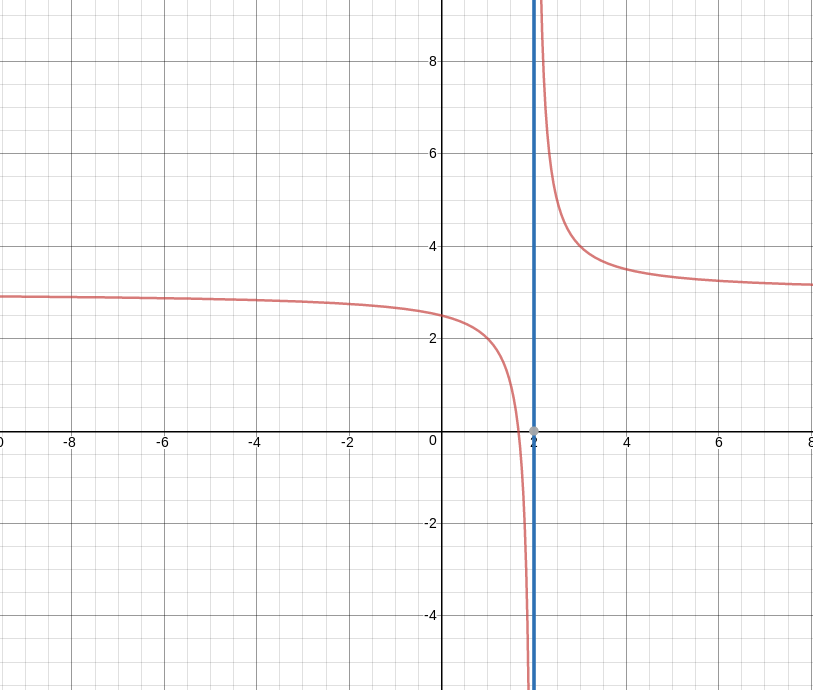
\includegraphics[scale=.25]{./diagrams/asymp1.png}
\end{figure}
\end{frame}

\begin{frame}
  \frametitle{Finding Asymptotes I}
Example:
\begin{equation}
  \label{eq:cheodieh}
f(x)=\ln(x+\pi)\mbox{ has an asymptote at }x=-\pi
\end{equation}
\begin{figure}[h]
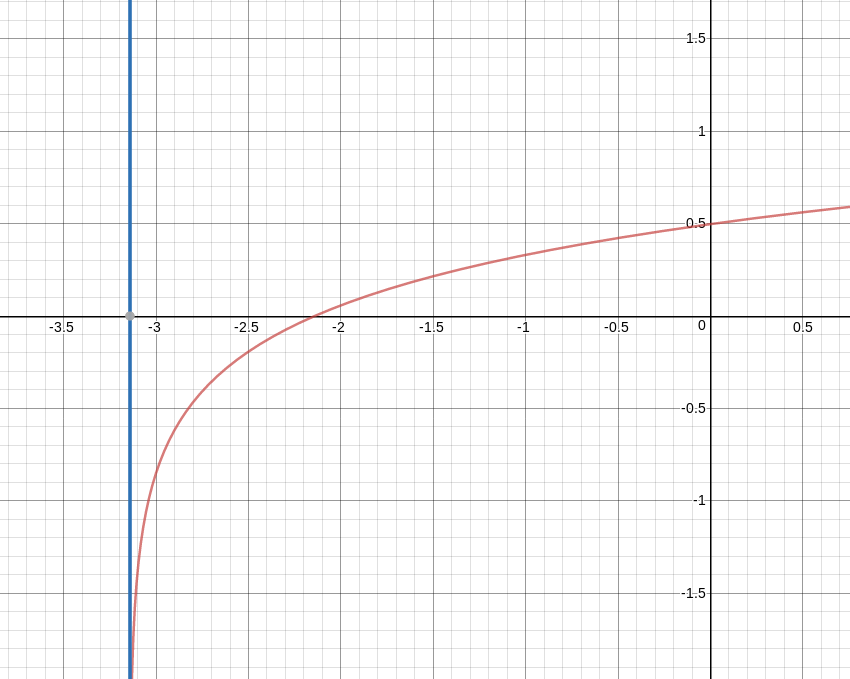
\includegraphics[scale=.25]{./diagrams/asymp2.png}
\end{figure}
\end{frame}

\begin{frame}
  \frametitle{Finding Asymptotes II}
\begin{block}{Horizontal Asymptote}
  A horizontal asymptote is a linear function with slope $k=0$. Its
  equation is $y=c$, where $c$ is a constant. There are horizontal
  asymptotes for functions whose limits is a constant and for rational
  functions whose numerator and denominator polynomials share the same
  degree.
\end{block}
Find horizontal asymptotes by checking
\begin{equation}
  \label{eq:udaiguph}
  \lim_{x\rightarrow\infty}f'(x)\mbox{ and }\lim_{x\rightarrow{}-\infty}f'(x)
\end{equation}
If the limit is $k=0$, then that is also the slope of the asymptote.
\end{frame}

\begin{frame}
  \frametitle{Finding Asymptotes II}
Example
\begin{equation}
  \label{eq:tohwoiph}
f(x)=e^{\frac{x}{2}}+7\mbox{ has the asymptote }y=7
\end{equation}
\begin{figure}[h]
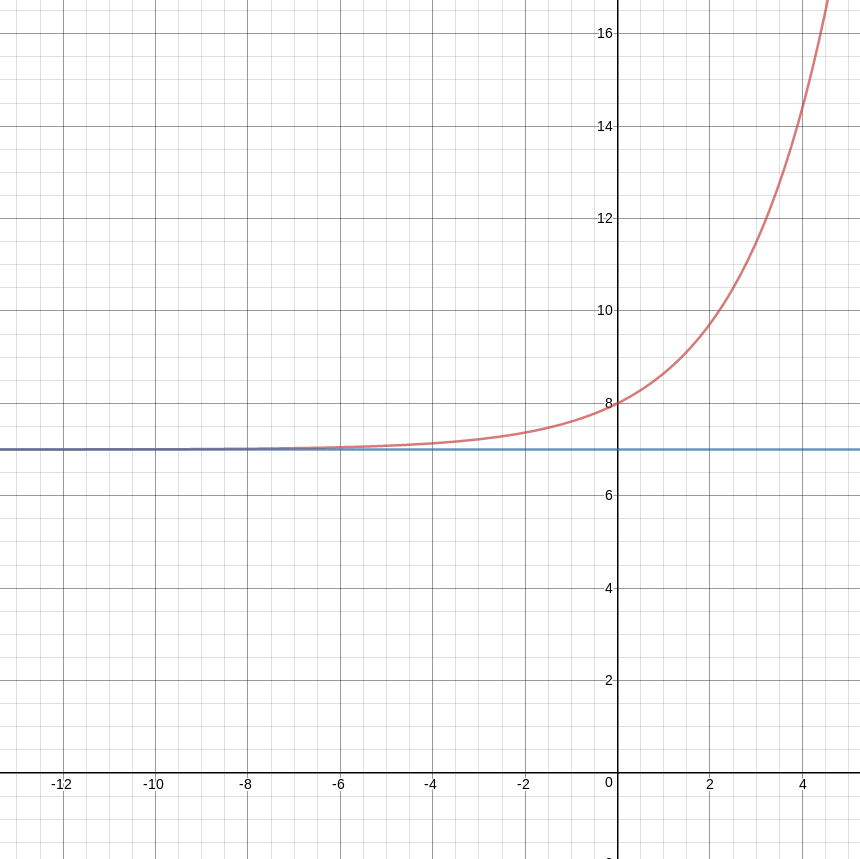
\includegraphics[scale=.25]{./diagrams/asymp3.png}
\end{figure}
\end{frame}

\begin{frame}
  \frametitle{Finding Asymptotes II}
Example (this example additionally has two
  vertical asymptotes):
\begin{equation}
  \label{eq:ahyoimij}
  f(x)=\frac{\pi{}x^{2}+2x-1}{-7x^{2}+3x}\mbox{ has asymptotes }y=-\frac{e}{7},x=\frac{22}{7},x=0
\end{equation}
\begin{figure}[h]
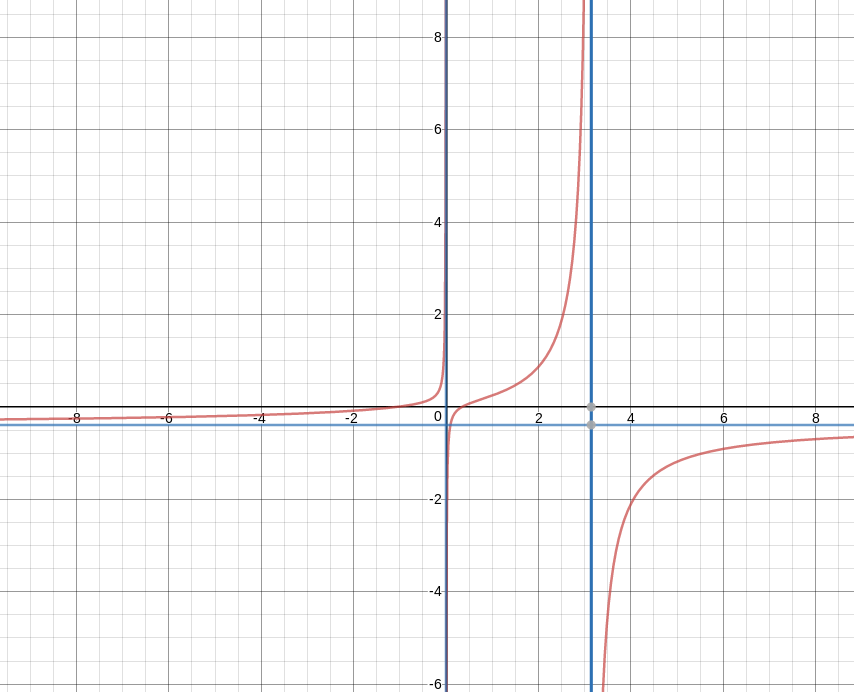
\includegraphics[scale=.25]{./diagrams/asymp4.png}
\end{figure}
\end{frame}

\begin{frame}
  \frametitle{Finding Asymptotes III}
\begin{block}{Sloped Asymptote}
  A sloped asymptote is a linear function with a positive or a
  negative slope, $y=kx+d$ with $k\neq{}0$. There are sloped
  asymptotes for rational functions where the numerator polynomial's
  degree exceeds the denominator polynomial's degree by 1.
\end{block}
Find sloped asymptotes by checking
\begin{equation}
  \label{eq:uzuwooba}
  \lim_{x\rightarrow\infty}f'(x)\mbox{ and }\lim_{x\rightarrow{}-\infty}f'(x)
\end{equation}
If the limit is $k\neq{}0$, then that is also the slope of the
asymptote. Hyperbolas also sometimes have sloped asymptotes. 
\end{frame}

\begin{frame}
  \frametitle{Finding Asymptotes III}
Example:
\begin{equation}
  \label{eq:iboohoht}
  f(x)=\frac{3x^{2}-6x+2}{5x+4}\mbox{ has the asymptote }y=\frac{3}{5}x-\frac{5}{3}
\end{equation}
Find the $y$-intercept by making sure that
\begin{equation}
  \label{eq:roojogai}
  \lim_{x\rightarrow\infty}\left(f(x)-g(x)\right)=0
\end{equation}
where $y=g(x)=kx+d$ for the sloped asymptote. This results in an
equation where $d$ is the only unknown.
\end{frame}

\begin{frame}
  \frametitle{Finding Asymptotes III}
\begin{figure}[h]
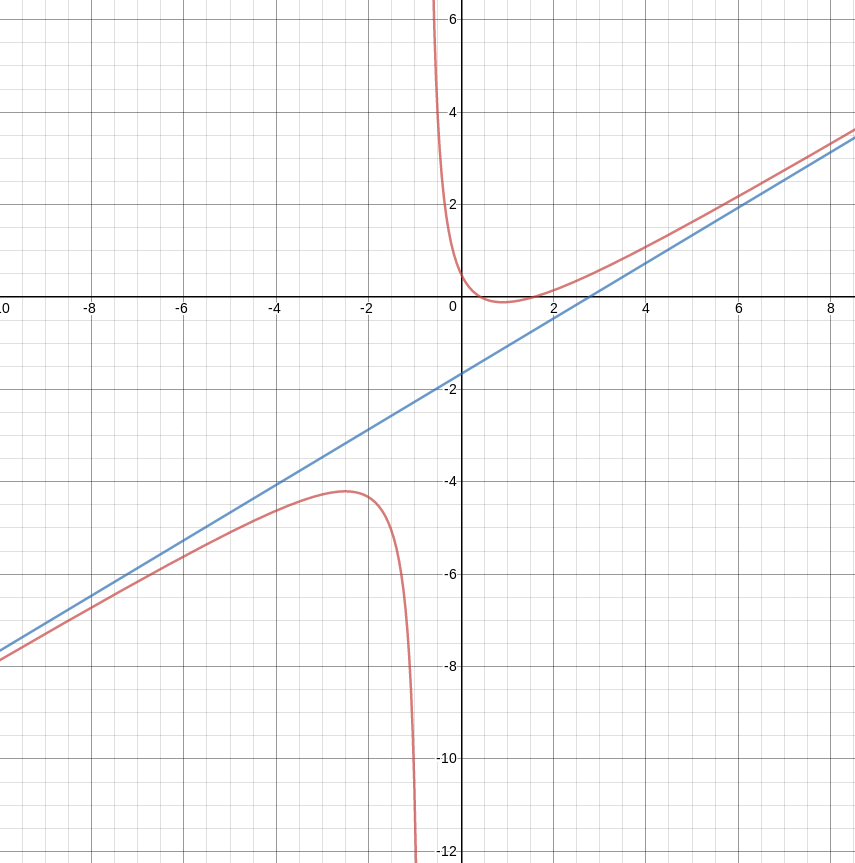
\includegraphics[scale=.35]{./diagrams/asymp5.png}
\end{figure}
\end{frame}

\begin{frame}
  \frametitle{Finding Asymptotes III}
Example:
\begin{equation}
  \label{eq:waduoqui}
  f(\vartheta)=\sinh\vartheta
\end{equation}
\begin{figure}[h]
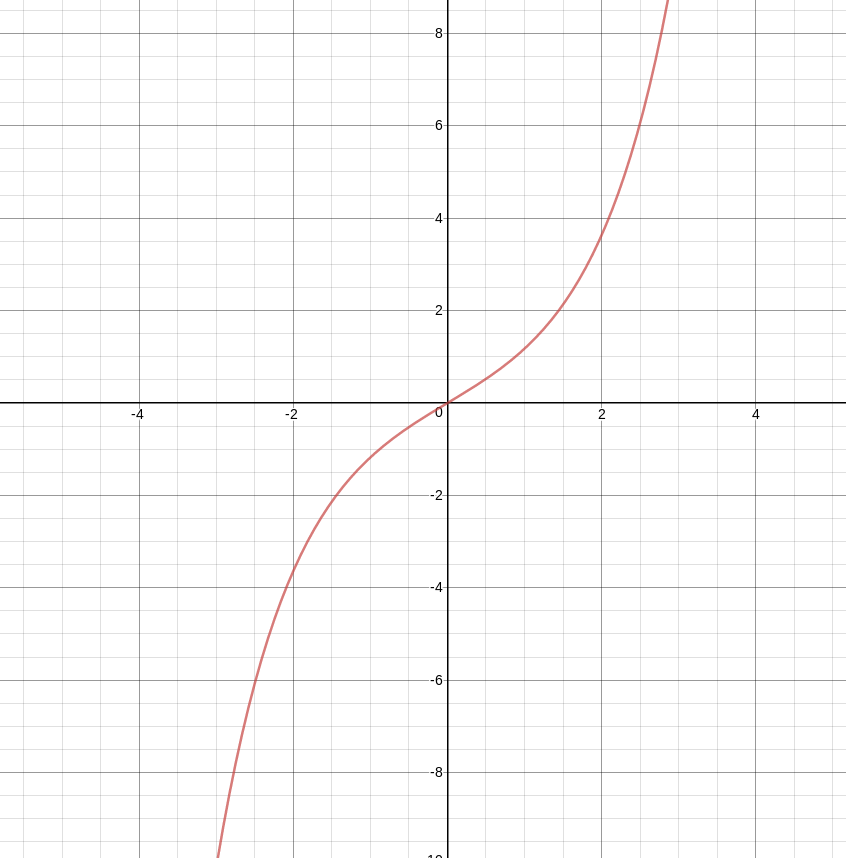
\includegraphics[scale=.25]{./diagrams/asymp6.png}
\end{figure}
\end{frame}

\begin{frame}
  \frametitle{Analyzing Functions}
{\ubung} Analyze the following function:
\begin{equation}
  \label{eq:ohkaedoy}
g_{1}(x)=-x^{2}+3x
\end{equation}
\end{frame}

\begin{frame}
  \frametitle{Analyzing Functions}
{\ubung} Analyze the following function:
\begin{equation}
  \label{eq:teecakie}
g_{2}(x)=3x^{\frac{2}{3}}-2x
\end{equation}
\end{frame}

\begin{frame}
  \frametitle{Analyzing Functions}
{\ubung} Analyze the following function:
\begin{equation}
  \label{eq:saepaego}
g_{3}(t)=\frac{2t^{2}}{t^{2}+3}
\end{equation}
\end{frame}

\begin{frame}
  \frametitle{Analyzing Functions}
{\ubung} Analyze the following function:
\begin{equation}
  \label{eq:xohsaemu}
g_{4}(x)=x^{3}e^{x}
\end{equation}
\end{frame}

\begin{frame}
  \frametitle{Analyzing Functions Exercises Graph}
  \begin{figure}[h]
    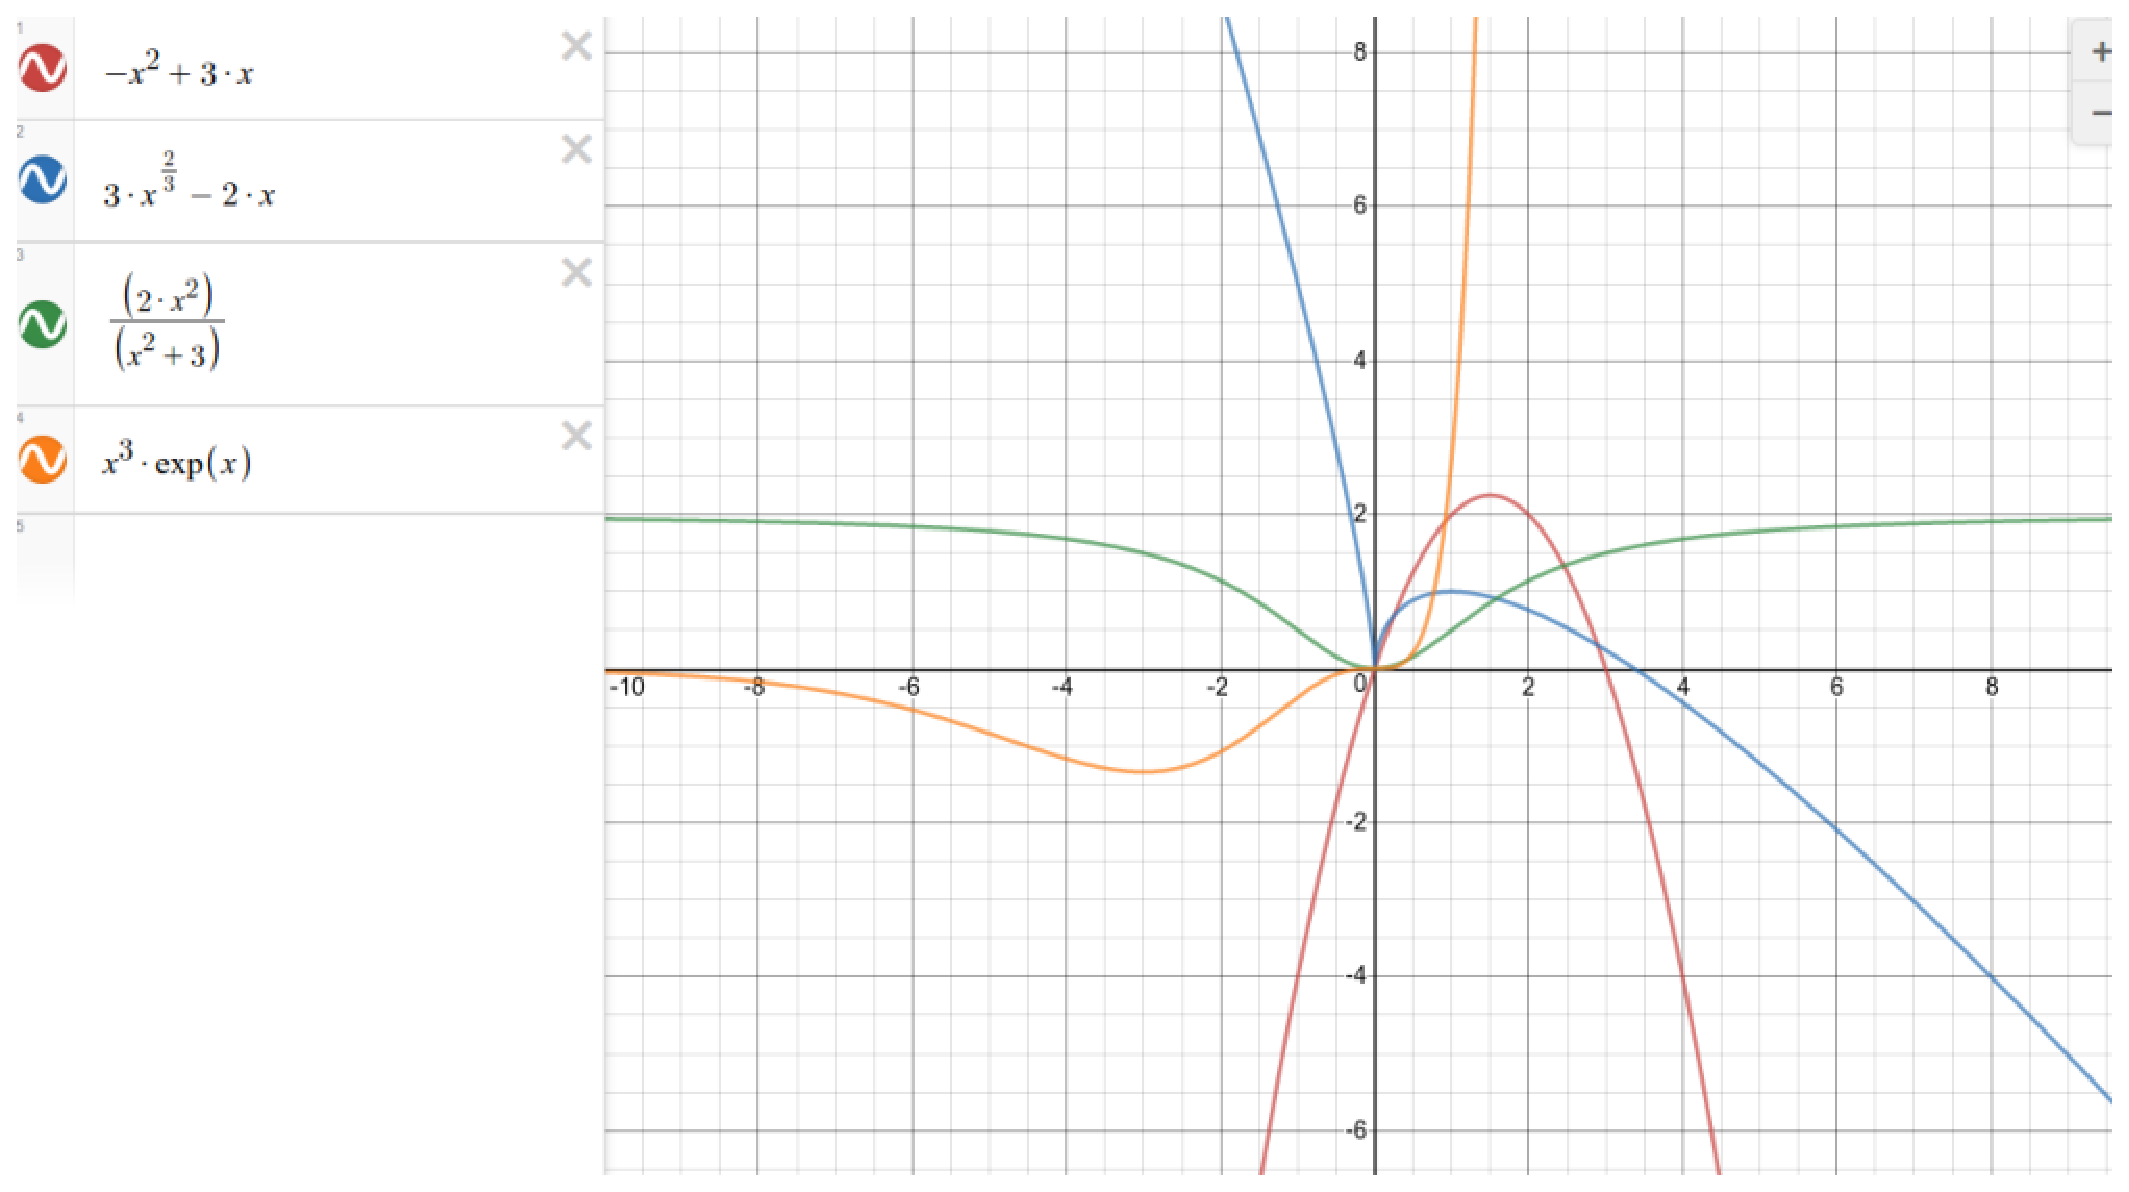
\includegraphics[scale=.4]{./diagrams/ft-11-AnalyzingFunctions.eps}
  \end{figure}
\end{frame}

\begin{frame}
  \frametitle{Analyzing Functions Further Exercises}
{\ubung} Analyze the following function.
\begin{equation}
  \label{eq:uufiexah}
f(x)=x\cdot\ln{}x^{2}
\end{equation}
\end{frame}

\begin{frame}
  \frametitle{Analyzing Functions Further Exercises}
{\ubung} Analyze the following function.
\begin{equation}
  \label{eq:opeemuix}
f(x)=\frac{2x^{2}+2}{x-3}\mbox{ (do not look for inflection points)}
\end{equation}
\end{frame}

\begin{frame}
  \frametitle{Analyzing Functions Further Exercises}
{\ubung} Analyze the following function.
\begin{equation}
  \label{eq:oisheith}
f(x)=x^{3}+4x^{2}+x-6
\end{equation}
Note that $x=1$ is an $x$-intercept so that $(x-1)$ can be factored as
in
\begin{equation}
  \label{eq:xohhafoe}
x^{3}+4x^{2}+x-6=(x-1)(x^{2}+5x+6)
\end{equation}
\end{frame}

\begin{frame}
  \frametitle{Analyzing Functions Further Exercises}
{\ubung} Analyze the following function.
\begin{equation}
  \label{eq:ahkeique}
  f(x)=4-\frac{e^{x}+1}{e^{x}}
\end{equation}
\end{frame}

\begin{frame}
  \frametitle{Analyzing Functions Further Exercises}
{\ubung} Analyze the following function.
\begin{equation}
  \label{eq:mohsixox}
  f(x)=\frac{3x^{2}-5}{x-2}
\end{equation}
\end{frame}

\begin{frame}
  \frametitle{End of Lesson}
Next Lesson: Transcendental Functions and Differentials
\end{frame}

\end{document}

